\section{Experimental Setup}\label{sec:setup}

\subsection{Datasets}\label{sec:setup-data}

The LTA collection contains 15,316 images from eight Singapore cameras over two
weeks, sampled at ten-minute intervals
\parencite{ltatrafficimages2026}.\footnote{The project image collection and the
human-corrected annotation subset are distributed as the
\href{https://huggingface.co/datasets/LOVEIII486/isy5002-lta-traffic-images}{LTA
image dataset on Hugging Face}; annotations are under
\texttt{annotations/lta\_human\_v1/}. The images remain under the Singapore Open
Data Licence 1.0; the annotations are released under CC BY 4.0.}
Week~1 and week~2 are disjoint in time.
For detection fine-tuning, 240 week-1 images are used for training and 80
week-2 images for validation, stratified by camera and by Singapore-time
day/night. The 240 training images also provide the pseudo-labeled
target-domain set used in joint fine-tuning. The labels are generated from
these images by YOLO26x; they are derived labels generated within the project.
Nighttime frames are a particular constraint: vehicles are small and poorly
lit, and even human annotation is difficult. Teacher labels and human labels
collected at night are therefore the least reliable reference.
Figure~\ref{fig:detection-examples} shows representative frames and labels from
both detection datasets.

MIO-TCD provides the human-labeled detection benchmark
\parencite{luo2018miotcd}.\footnote{The MIO-TCD localization dataset is
available at \url{https://tcd.miovision.com/}; paper DOI:
\url{https://doi.org/10.1109/TIP.2018.2848705}.}
Its localization set contains 137,743 annotated frames; the training release
used here contains 110,000 images. We map its eleven classes to four: work vans
to car; pickup, single-unit and articulated trucks to truck; bus and motorcycle
unchanged. Pedestrian, bicycle and non-motorized-vehicle boxes are dropped, and
images containing the class \texttt{motorized\_vehicle} (vehicles too small to
classify) are removed, leaving 89,701 images. Because many images are consecutive
frames from the same camera, we link images when they share a file hash, when
their 256-bit difference-hash distance is at most 16, when their background
thumbnails correlate at 0.95 or above, or when their vehicle-masked background
thumbnails correlate at 0.93 or above; connected components form 1,592 scene
groups. Whole groups are assigned to pools, and fixed-size samples are drawn
from the pools: 8,000 training images, 1,000 development images, 2,000 test
images and a 161-image motorcycle diagnostic split. The fixed caps keep the
30-epoch fine-tuning runs tractable and preserve rare-class coverage; the
remaining filtered images are not used. The test split contains 31 scene groups
and is evaluated once. Our splits are drawn from its training set; the official
test labels are not public.

PEMSD8 provides the forecasting benchmark: 170 sensors and 17,856 five-minute
observations. The series is distributed by LibCity \parencite{jiang2023libcity};
the raw measurements come from Caltrans PeMS.\footnote{Caltrans PeMS:
\url{https://pems.dot.ca.gov/}; LibCity dataset repository:
\url{https://github.com/LibCity/Bigscity-LibCity-Datasets}.}
The common protocol uses a 7:1:2 chronological split, 12 input steps and 12
output steps. The scaler is fitted on the training input windows, and the test
window indices are recorded for every run.
Figure~\ref{fig:pemsd8-series} shows a representative sensor series and its
daily profile.

COCO-pretrained weights provide model initialization. The datasets above supply
all training and evaluation data. Detection accuracy is measured on the
human-labeled MIO-TCD test set; on LTA, results are reported both against
teacher-generated labels and against human-corrected labels.

In addition, two human-annotated LTA sets are used. For detection accuracy and
the camera filter, an annotator corrected the boxes on the 80 week-2 validation
images; 17 images judged too difficult to label reliably were removed, leaving
63 images with 1,197 vehicle boxes. The annotations were initialized from
teacher pre-labels and are therefore human-corrected, not independent of the
teacher. For congestion, 600 frames
were labeled free-flowing, moderate or congested in a browser tool that outlines
the detection zones and hides the timestamp. The frames were drawn at random per
camera within five Singapore-time strata (weekday peak, weekday off-peak, weekend
day, evening and late night), never selected by any voter's score, and were split
before labeling into 25 practice and 50 test frames per camera. A frame skipped
as impossible to judge was replaced by a spare from the same camera and stratum.
The practice set contains 107 free-flowing, 47 moderate and 46 congested frames;
the test set contains 171, 127 and 102.

\begin{figure}[H]
  \centering
  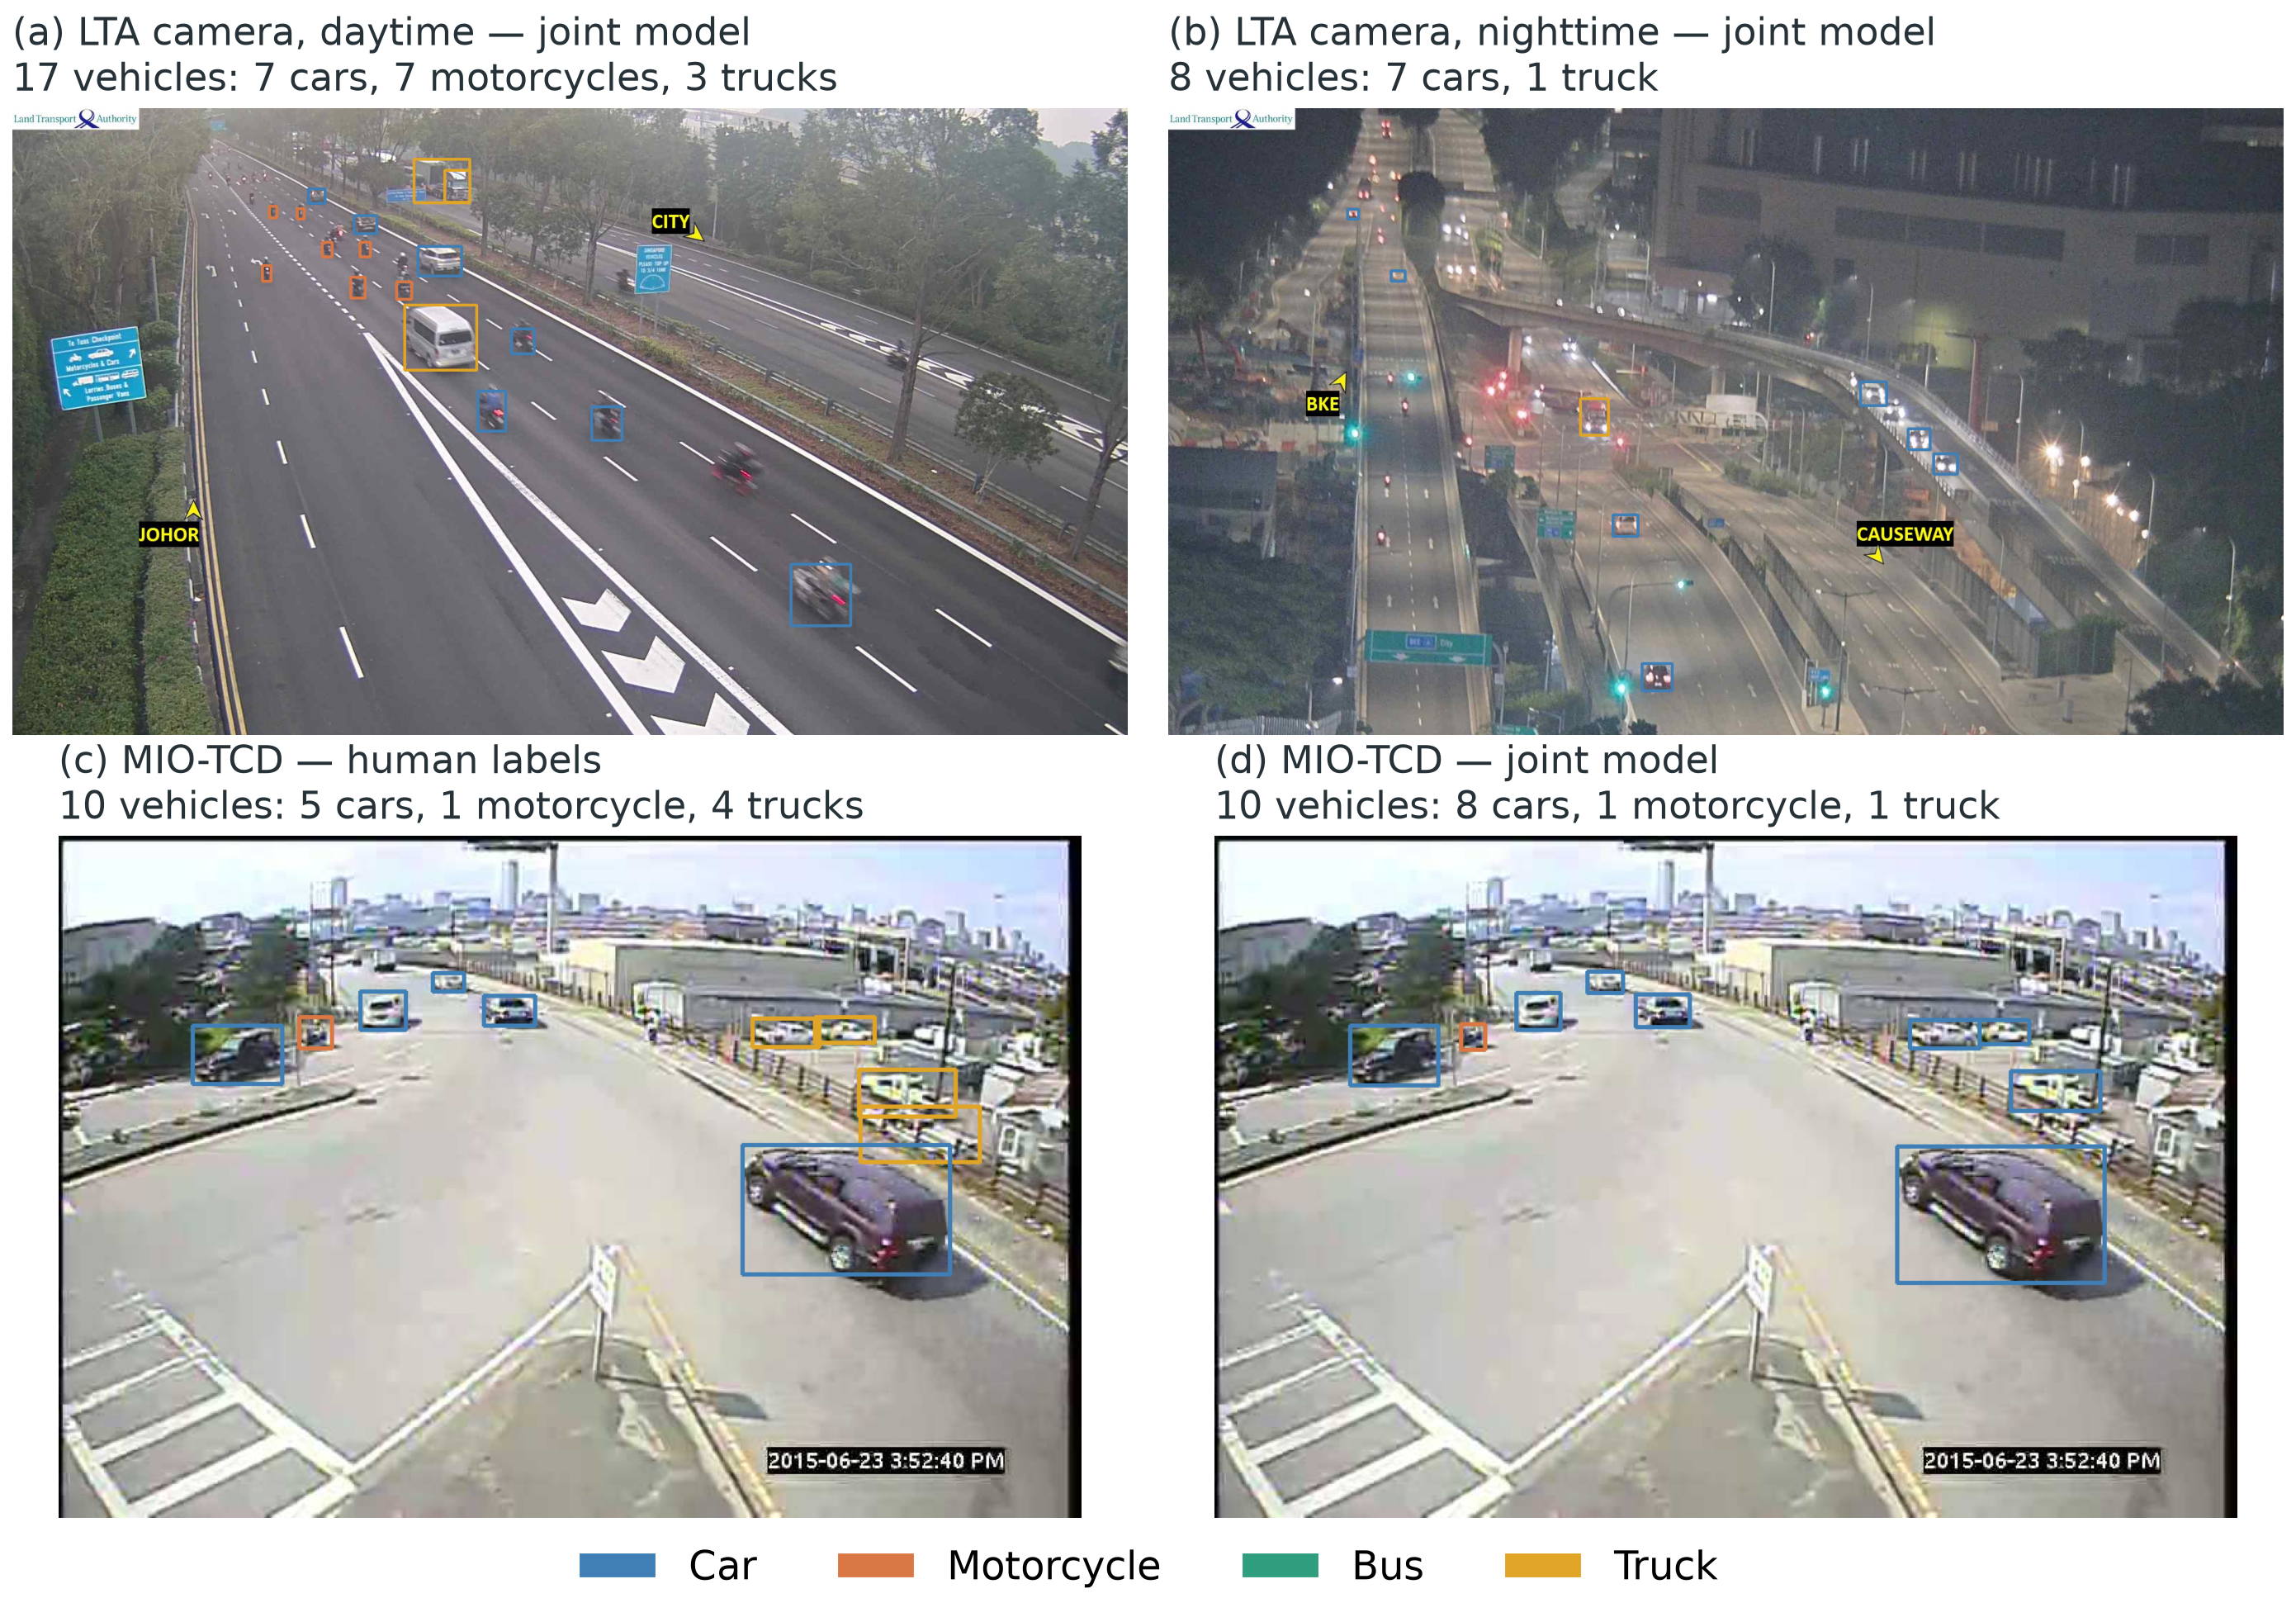
\includegraphics[width=0.92\linewidth]{detection_examples.png}
  \caption{Examples from the detection datasets. (a) LTA daytime and (b) LTA
  nighttime frames with joint-model detections; (c) a MIO-TCD test image with
  human labels; (d) the same image with joint-model detections. Box colors
  denote vehicle classes; titles report detected or labeled counts.}
  \label{fig:detection-examples}
\end{figure}

\begin{figure}[H]
  \centering
  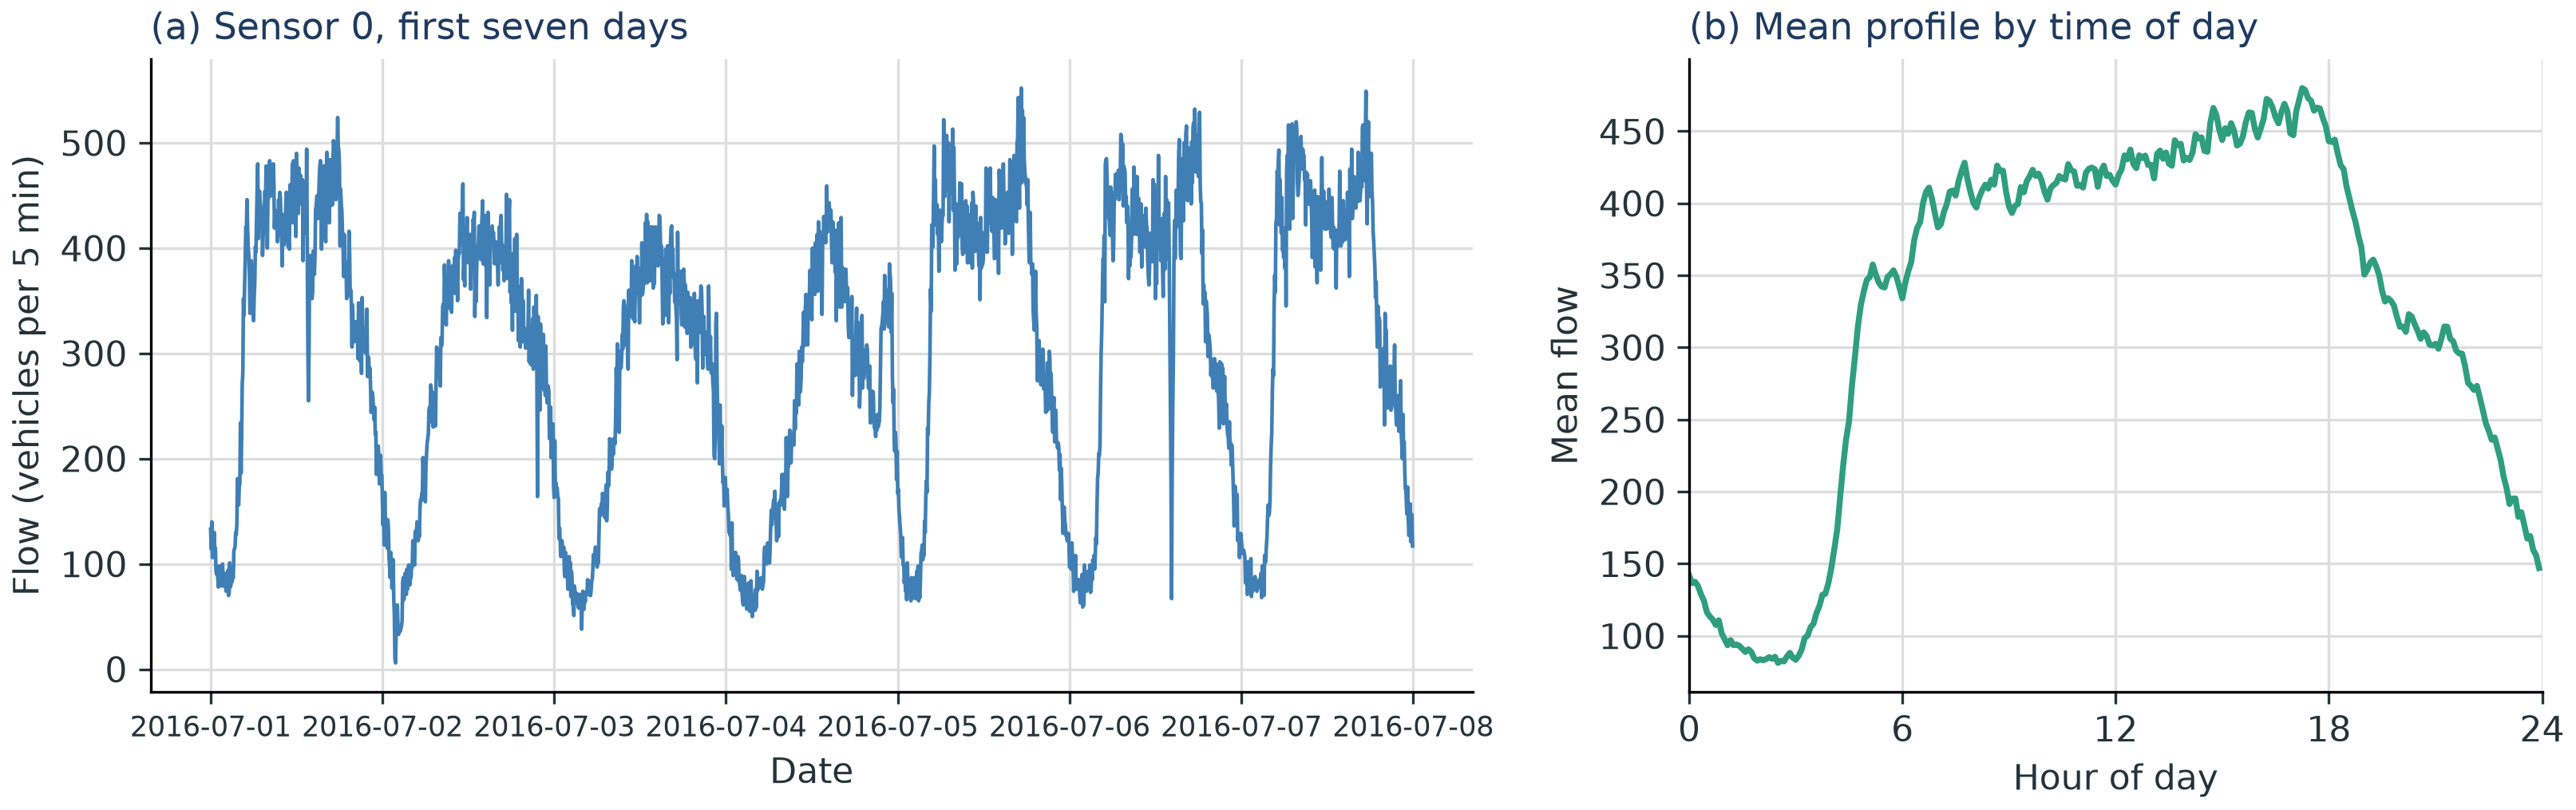
\includegraphics[width=\linewidth]{pemsd8_series.png}
  \caption{PEMSD8 traffic flow for sensor~0. (a) First seven days of the
  five-minute series; (b) mean flow by time of day over the full collection.
  The daily cycle motivates the time-of-day input used in the unified setting.}
  \label{fig:pemsd8-series}
\end{figure}

\subsection{Data Domains}\label{sec:setup-domains}

The prototype draws on two data sources. LTA images provide camera views and
per-frame vehicle counts. PEMSD8 provides calibrated flow, occupancy and speed
series for a road network. Each source supports one module: imagery for
recognition and calibrated series for forecasting. An end-to-end deployment
requires both at the same locations, aligned in time;
Section~\ref{sec:method-integration} defines this interface. The workbench presents
the two source-labeled views.

\subsection{Evaluation Protocol and Metrics}\label{sec:setup-metrics}

Detection is scored with COCO-style mAP \parencite{lin2014coco} at IoU~0.5 and
0.5:0.95, per-class AP, precision/recall at confidence~0.25, and mean absolute
counting error. Confidence intervals come from 2,000 bootstrap resamples of
scene groups; paired differences reuse the same resamples. This interval covers
scene sampling only, because each detector configuration was trained once.

The camera filter is scored on the 63 human-corrected images by class-agnostic
precision and recall at IoU~0.5 and confidence~0.25, before and after filtering,
with 2,000 bootstrap resamples of images. These intervals are image-level and do
not account for correlation between frames from the same camera, so they are
optimistic. Congestion levels are scored by
accuracy and linearly weighted Cohen's kappa \parencite{cohen1968kappa}, which
counts confusing free-flowing with congested as twice as severe as confusing
adjacent levels, together with precision and recall for the congested level.
Features, cut points and the primary method are chosen by five-fold
cross-validation repeated 20 times on the practice labels. The primary method is
the candidate with the highest cross-validated kappa; within 0.005 of the best,
the simpler candidate is preferred. The test labels are used once, after the
configuration is frozen, with 2,000 bootstrap resamples of test frames. These
intervals are frame-level; the 50 frames from each camera are correlated, so the
intervals are optimistic. Because peak hours are over-sampled, accuracy is also
reported with each test frame weighted by its camera and stratum's share of all
frames.

Forecasting uses masked MAE, RMSE and MAPE, averaged over the 12 output steps,
with 15/30/60-minute breakdowns at output steps 3, 6 and 12. MAE is measured in
vehicles per five-minute interval. Masked metrics ignore zero ground truth, with
a threshold of $10^{-4}$. The scaler is a standard scaler fitted on the training
input windows. All models use batch size 64, at most 100 epochs, early stopping
with patience 30, and checkpoint selection by validation loss; optimizer,
learning rate and schedule follow each model's LibCity default. Runs used
PyTorch on Apple MPS with LibCity commit \texttt{5a6391d}. Seeds control
initialization, shuffling and dropout, while data splits and test windows are
fixed. Forecast intervals are paired $t$-intervals over seeds, not bootstrap
intervals; the five-seed results are reported separately.
